\section{Configuration de l'environnement de développement embarqué}

Le développement du firmware pour le microcontrôleur gérant transmission (STM32) repose sur 
le kit de développement logiciel officiel de Morse Micro (\texttt{mm-iot-sdk}). Ce SDK étant 
nativement conçu pour un environnement Linux avec platformio et des chaînes de cross compilation 
préinstallées, son intégration sous Windows a nécessité plusieurs adaptations.



\subsection{Intégration du SDK sous Windows}
Le code source a été récupéré via le dépôt GitHub officiel. L'architecture du projet s'appuyant sur 
plusieurs dépendances externes vitales (telles que le système d'exploitation temps réel 
FreeRTOS\index{FreeRTOS}, la pile réseau LwIP\index{LwIP} et mbedTLS), une initialisation complète des 
sous-modules a été requise (git submodules).

L'environnement de développement choisi est \textbf{STM32CubeIDE}\index{STM32CubeIDE}. Le SDK ne 
respectant pas la structure standard de cet IDE, le projet a été importé en tant que "Makefile 
Project with Existing Code", en ciblant spécifiquement le répertoire de la carte d'évaluation de 
l'émetteur (\texttt{mm-mm6108-ekh05}, avant sa mise à jour, \texttt{mm-mm8108-ekh05} après).

\subsection{Adaptation de la chaîne de cross compilation}
Sous Windows, les outils de compilation en ligne de commande tels que \texttt{make} ne sont pas natifs. 
Pour pallier ce problème, les variables d'environnement du projet dans STM32CubeIDE ont été modifiées 
pour inclure les chemins absolus vers les utilitaires internes de l'IDE (\texttt{make.exe} et 
\texttt{arm-none-eabi-gcc.exe}).

De plus, le SDK force la recherche de la chaîne de compilation GCC ARM dans les répertoires 
typiques de Linux (tels que \texttt{/opt/}). Il a donc été nécessaire de modifier le fichier de configuration 
principal \texttt{mkcore-arm-cortex-m33f.mk} pour empêcher cette recherche et permettre au système d'utiliser 
le \texttt{PATH} de Windows :

\begin{lstlisting}[language=make]
# --- MODIFICATION POUR WINDOWS / STM32CubeIDE ---
# On ignore la recherche des dossiers Linux /opt/...
# et on laisse le PATH systeme de STM32CubeIDE trouver le compilateur.
TOOLCHAIN_DIR := 
TOOLCHAIN_BASE := arm-none-eabi-

CC := "$(TOOLCHAIN_BASE)gcc"
CXX := "$(TOOLCHAIN_BASE)g++"
AS := $(CC) -x assembler-with-cpp
OBJCOPY := "$(TOOLCHAIN_BASE)objcopy"
\end{lstlisting}

\subsection{Configuration du débogage matériel (ST-LINK)}
Pour permettre l'exécution pas à pas et la pose de breakpoint, le projet a été converti en "Projet ARM" 
dans l'IDE. La sonde de débogage utilisée est le \textbf{ST-LINK}\index{ST-LINK} intégré à la carte 
EKH05, communiquant via le protocole SWD (\textit{Serial Wire Debug}).

% PLACEHOLDER POUR LE SCHEMA OU CAPTURE D'ECRAN
\begin{figure}[htbp]
    \centering
    % 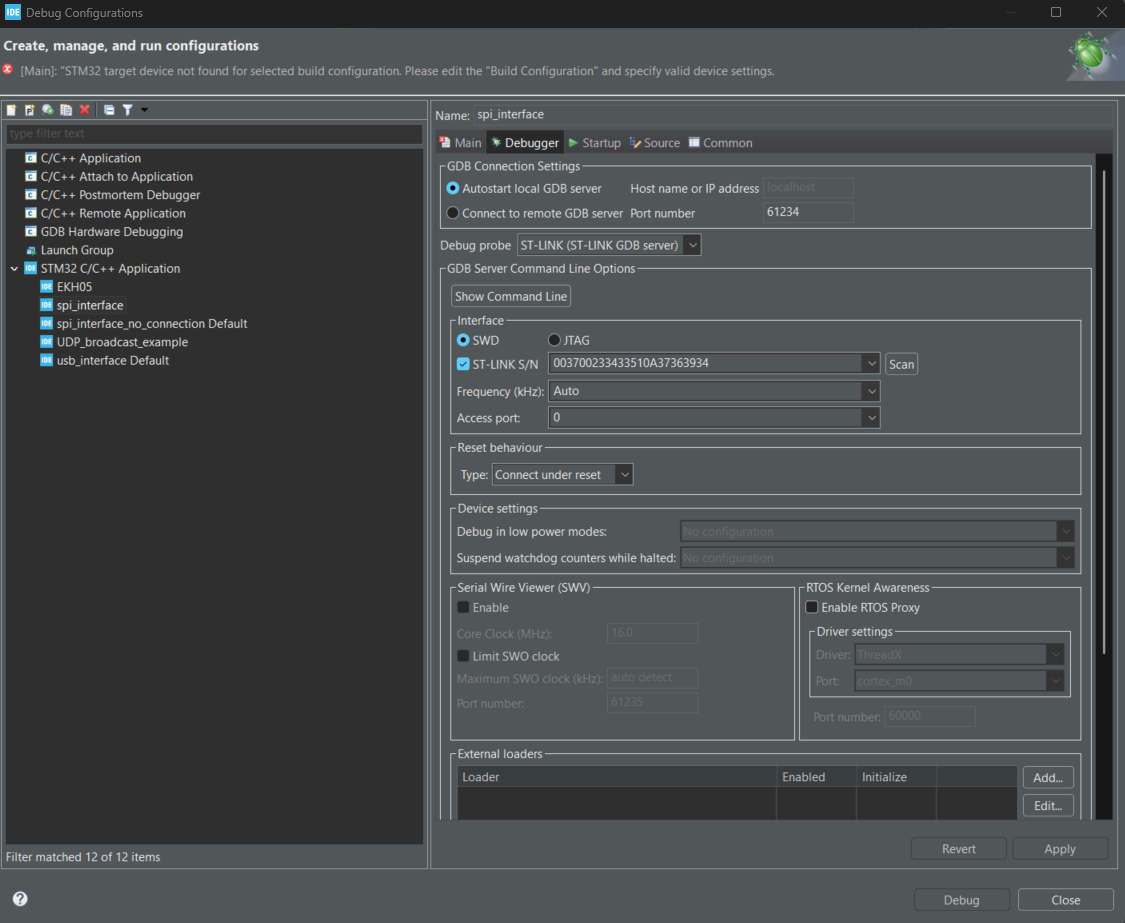
\includegraphics[width=0.8\textwidth]{imgs/debug_config_cubeide.png}
    \caption{Configuration du serveur GDB ST-LINK dans STM32CubeIDE}
    \label{fig:debug_config}
\end{figure}

Il est important de noter une limitation physique de cette architecture : la sonde USB (ST-LINK) ne peut 
maintenir qu'un seul tunnel de communication actif à la fois. L'utilisation simultanée de la console 
série (ex: PuTTY,Termite) et du débogueur GDB entraîne des conflits matériels.

\subsection{Provisionnement et calibration radio (Config Store)}
Une étape indispensable, distincte de la compilation du code C, est le \textbf{provisionnement} de la puce 
Wi-Fi. La puce Morse Micro ne possède pas de mémoire non volatile interne pour ses paramètres vitaux ; 
elle ne peut pas démarrer sans son micro-code (BCF) et ses paramètres régionaux (\textit{Country Code}), 
stockés dans une zone mémoire spécifique du STM32 appelée le \textit{Config Store}.

\subsubsection{Architecture de flashage}
Le processus de flashage repose sur une architecture client-serveur :
\begin{enumerate}
    \item \textbf{Le Serveur (OpenOCD\index{OpenOCD}) :} Il établit la connexion matérielle entre le 
    port USB et le processeur ARM via la sonde ST-LINK.
    \item \textbf{Le Client (Script Python) :} Il lit le fichier de configuration utilisateur 
    (\texttt{config.hjson}), génère le binaire correspondant, et commande au serveur de l'écrire dans 
    la mémoire Flash du STM32 (à l'adresse \texttt{0x08004000}).
\end{enumerate}

\subsubsection{Résolution du conflit de signature et de version matérielle}
Lors des premiers déploiements, une erreur bloquait la communication SPI entre le MCU et la 
puce Wi-Fi (\texttt{Transport init failed - Chip ID 0x0000}). Le code embarqué plantait dès 
l'initialisation du HAL.

L'analyse de ce blocage a révélé un désaccord matériel : le code C et le fichier de 
configuration cachaient une dépendance stricte à l'ancienne plateforme (MM6108). Notre matériel étant la 
version MM8108, le binaire de calibration injecté était incorrect. Par une coïncidence extrêmement heureuse, 
Morse Micro a mis à jour son SDK public la semaine suivante, ajoutant officiellement 
le support de la cible \texttt{mm-mm8108-ekh05}. \newline

Cette mise à jour a permis de rediriger le script vers le fichier de calibration 
exact de la puce (\texttt{bcf\_mf08651\_us.mbin}). Combiné à l'ajustement du fichier \texttt{config.hjson} 
pour cibler la région "US", la puce radio a pu démarrer avec succès.\newline

Le module a été sciemment configuré pour cibler la région "US" (États-Unis, norme FCC sur la bande 
des 915 MHz) au lieu du domaine européen par défaut (norme ETSI sur la bande des 868 MHz). Ce choix 
est basé par les contraintes de partage du spectre radio. La réglementation européenne impose des 
règles strictes telles que le \textit{Listen Before Talk} (LBT) et des limites sévères de 
\textit{Duty Cycle} (temps de transmission maximal). Ces mécanismes forcent le module radio à 
retenir ou espacer ses paquets pour écouter si le canal est libre. \newline

Lors de nos tests initiaux, ces bridages réglementaires faisaient exploser la latence réseau 
de base à environ 670 ms. Le passage sur le standard américain permet de désactiver ces restrictions 
d'émission. Bien que cette configuration soit réservée à un cadre expérimental, elle était i
ndispensable pour ce travail de Bachelor afin de mesurer les performances brutes et réelles de 
la puce (ramenant la latence radio autour de 3 à 5 ms, tester par ping), indépendamment des 
limitations légales.